\begin{figure}
    \tiny
    \centering
    \begin{subfigure}{0.24\textwidth}
        \centering
        \begin{center}
            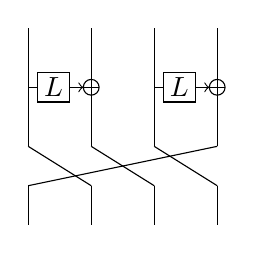
\begin{tikzpicture}[xscale=0.8, yscale=-0.5]
                \draw (0,0) -- (0,3);
                \draw (1,0) -- (1,3);
                \draw (2,0) -- (2,3);
                \draw (3,0) -- (3,3);
                \draw (0,4) -- (0,5);
                \draw (1,4) -- (1,5);
                \draw (2,4) -- (2,5);
                \draw (3,4) -- (3,5);
                \draw (0,3) -- (1,4);
                \draw (1,3) -- (2,4);
                \draw (2,3) -- (3,4);
                \draw (3,3) -- (0,4);
                \draw (1,1.5) ellipse (0.125 and 0.2);
                \draw (1,1.3) -- (1,1.7);
                \draw (0.875,1.5) -- (1.125,1.5);
                \draw (0,1.5) -- (0.15,1.5);
                \draw (0.15,1.125) rectangle (0.65,1.875) node[pos=0.5] {$L$};
                \draw [->] (0.65,1.5) -- (0.875,1.5);
                \draw (3,1.5) ellipse (0.125 and 0.2);
                \draw (3,1.3) -- (3,1.7);
                \draw (2.875,1.5) -- (3.125,1.5);
                \draw (2,1.5) -- (2.15,1.5);
                \draw (2.15,1.125) rectangle (2.65,1.875) node[pos=0.5] {$L$};
                \draw [->] (2.65,1.5) -- (2.875,1.5);
            \end{tikzpicture}
            \FigDef{best-layers-a}{}
        \end{center}
    \end{subfigure}
    \begin{subfigure}{0.24\textwidth}
    \centering
        \begin{center}
            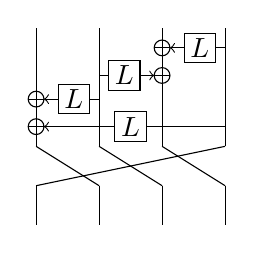
\begin{tikzpicture}[xscale=0.8, yscale=-0.5]
                \draw (0,0) -- (0,3);
                \draw (1,0) -- (1,3);
                \draw (2,0) -- (2,3);
                \draw (3,0) -- (3,3);
                \draw (0,4) -- (0,5);
                \draw (1,4) -- (1,5);
                \draw (2,4) -- (2,5);
                \draw (3,4) -- (3,5);
                \draw (0,3) -- (1,4);
                \draw (1,3) -- (2,4);
                \draw (2,3) -- (3,4);
                \draw (3,3) -- (0,4);
                \draw (2,1.2) ellipse (0.125 and 0.2);
                \draw (2,1) -- (2,1.4);
                \draw (1.875,1.2) -- (2.125,1.2);
                \draw (1,1.2) -- (1.15,1.2);
                \draw (1.15,0.825) rectangle (1.65,1.575) node[pos=0.5] {$L$};
                \draw [->] (1.65,1.2) -- (1.875,1.2);
                \draw (0,1.8) ellipse (0.125 and 0.2);
                \draw (0,1.6) -- (0,2);
                \draw (-0.125,1.8) -- (0.125,1.8);
                \draw (1,1.8) -- (0.85,1.8);
                \draw (0.35,1.425) rectangle (0.85,2.175) node[pos=0.5] {$L$};
                \draw [->] (0.35,1.8) -- (0.125,1.8);
                \draw (2,0.5) ellipse (0.125 and 0.2);
                \draw (2,0.3) -- (2,0.7);
                \draw (1.875,0.5) -- (2.125,0.5);
                \draw (3,0.5) -- (2.85,0.5);
                \draw (2.35,0.125) rectangle (2.85,0.875) node[pos=0.5] {$L$};
                \draw [->] (2.35,0.5) -- (2.125,0.5);
                \draw (0,2.5) ellipse (0.125 and 0.2);
                \draw (0,2.3) -- (0,2.7);
                \draw (-0.125,2.5) -- (0.125,2.5);
                \draw (3,2.5) -- (1.75,2.5);
                \draw (1.25,2.125) rectangle (1.75,2.875) node[pos=0.5] {$L$};
                \draw [->] (1.25,2.5) -- (0.125,2.5);
            \end{tikzpicture}
            \FigDef{best-layers-b}{}
        \end{center}
    \end{subfigure}
    \begin{subfigure}{0.24\textwidth}
        \centering
        \begin{center}
            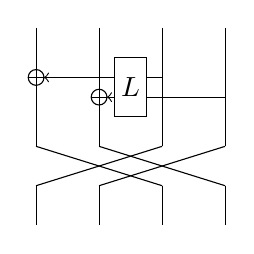
\begin{tikzpicture}[xscale=0.8, yscale=-0.5]
                \draw (0,0) -- (0,3);
                \draw (1,0) -- (1,3);
                \draw (2,0) -- (2,3);
                \draw (3,0) -- (3,3);
                \draw (0,4) -- (0,5);
                \draw (1,4) -- (1,5);
                \draw (2,4) -- (2,5);
                \draw (3,4) -- (3,5);
                \draw (0,3) -- (2,4);
                \draw (1,3) -- (3,4);
                \draw (2,3) -- (0,4);
                \draw (3,3) -- (1,4);
                \draw (0,1.25) ellipse (0.125 and 0.2);
                \draw (0,1.05) -- (0,1.45);
                \draw (-0.125,1.25) -- (0.125,1.25);
                \draw (1,1.75) ellipse (0.125 and 0.2);
                \draw (1,1.55) -- (1,1.95);
                \draw (0.875,1.75) -- (1.125,1.75);
                \draw (2,1.25) -- (1.75,1.25);
                \draw (3,1.75) -- (1.75,1.75);
                \draw (1.25,0.75) rectangle (1.75,2.25) node[pos=0.5] {$L$};
                \draw [->] (1.25,1.25) -- (0.125,1.25);
                \draw [->] (1.25,1.75) -- (1.125,1.75);
            \end{tikzpicture}
            \FigDef{best-layers-c}{}
        \end{center}
    \end{subfigure}
    \begin{subfigure}{0.24\textwidth}
        \centering
        \begin{center}
            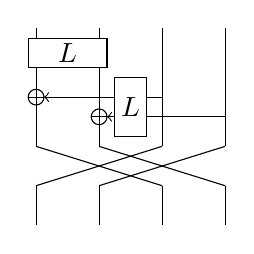
\begin{tikzpicture}[xscale=0.8, yscale=-0.5]
                \draw (2,0) -- (2,3);
                \draw (3,0) -- (3,3);
                \draw (0,4) -- (0,5);
                \draw (1,4) -- (1,5);
                \draw (2,4) -- (2,5);
                \draw (3,4) -- (3,5);
                \draw (0,0) -- (0,0.25);
                \draw (1,0) -- (1,0.25);
                \draw (-0.125,0.25) rectangle (1.125,1) node[pos=0.5] {$L$};
                \draw (0,1) -- (0,3);
                \draw (1,1) -- (1,3);
                \draw (0,3) -- (2,4);
                \draw (1,3) -- (3,4);
                \draw (2,3) -- (0,4);
                \draw (3,3) -- (1,4);
                \draw (0,1.75) ellipse (0.125 and 0.2);
                \draw (0,1.55) -- (0,1.95);
                \draw (-0.125,1.75) -- (0.125,1.75);
                \draw (1,2.25) ellipse (0.125 and 0.2);
                \draw (1,2.05) -- (1,2.45);
                \draw (0.875,2.25) -- (1.125,2.25);
                \draw (2,1.75) -- (1.75,1.75);
                \draw (3,2.25) -- (1.75,2.25);
                \draw (1.25,1.25) rectangle (1.75,2.75) node[pos=0.5] {$L$};
                \draw [->] (1.25,1.75) -- (0.125,1.75);
                \draw [->] (1.25,2.25) -- (1.125,2.25);
            \end{tikzpicture}
            \FigDef{best-layers-d}{}
        \end{center}
    \end{subfigure}
    \FigDef{best-layers}{Possible linear layers.} 
\end{figure}